%auto-ignore
\documentclass[tikz]{standalone}

\usetikzlibrary{calc}

\usepackage{mathdots}

\begin{document}
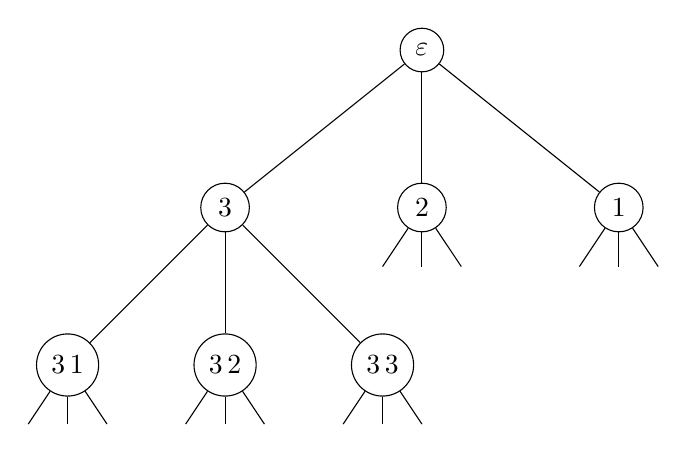
\begin{tikzpicture}[scale=0.5]

\node [circle,draw=black] (n) at (0,0) {$\varepsilon$};

\node [circle,draw=black] (n1) at (-5,-4) {$3$};
\node [circle,draw=black] (n2) at ( 0,-4) {$2$};
\node [circle,draw=black] (nd) at ( 5,-4) {$1$};

%\node at ($(n2)!0.5!(nd)$) {$\cdots$};

\node [circle,draw=black] (n11) at ( -9,-8) {$3 \, 1$};
\node [circle,draw=black] (n12) at ( -5,-8) {$3 \, 2$};
\node [circle,draw=black] (n1d) at ( -1,-8) {$3 \, 3$};

%\node at ($(n12)!0.5!(n1d)$) {$\cdots$};

\draw (n) to (n1);
\draw (n) to (n2);
\draw (n) to (nd);


\draw (n1) to (n11);
\draw (n1) to (n12);
\draw (n1) to (n1d);

\foreach \i in {11,12,1d,2,d} {
\draw [] (n\i) to +(-1,-1.5);
\draw [] (n\i) to +( 0,-1.5);
\draw [] (n\i) to +( 1,-1.5);
%\node at ($(n\i)+(0.45,-1.4)$) {\tiny$\cdots$};
}

\end{tikzpicture}
\end{document}